\documentclass[11pt, a4paper]{article}
\usepackage[utf8]{inputenc}
\usepackage[margin=1in]{geometry} %Sets proper 1-inch margins. 
\usepackage{amsmath} %Only load this if you are using math/equations.
\usepackage{graphicx} %Only need to call this if inserting images.
\usepackage{caption} %Only need to call this if inserting captions.
\usepackage{float} %Allows the use of the [H] specifier. 
\graphicspath{{C:/Users/jonah/Pictures/meme/}} %Sets the working directory for images.
\usepackage[colorlinks,citecolor=blue,linkcolor=blue,urlcolor=blue]{hyperref} %Allows for the embedding of urls. 
\usepackage{setspace}
\usepackage{blindtext}

\pagenumbering{arabic}

\usepackage{fancyhdr}

\pagestyle{fancy}
\fancyhf{}
\rhead{Jonah Edmundson \\ 2023}
\lhead{\thepage}

\newcommand{\comment}[1]{}

\usepackage{Sweave}
\begin{document}
\Sconcordance{concordance:variableinvestigation.tex:variableinvestigation.Rnw:%
1 23 1 1 0 19 1 1 2 1 0 3 1 1 6 5 0 1 3 1 0 1 3 1 0 1 12 14 0 1 2 8 1 1 %
3 2 0 1 2 1 0 1 2 1 0 1 2 6 0 1 6 9 0 1 2 3 1 1 4 3 0 1 2 8 0 1 7 9 0 1 %
2 6 1 1 2 1 0 1 7 9 0 1 2 1 5 10 0 1 8 11 0 1 2 2 1 1 14 17 0 1 2 30 1}


\begin{center}
\Large{\textsc{Variable Investigation}}
\par
\normalsize{\textsc{for}}
\par
\large{\textsc{Kelowna Weather-Crash Project}}
\end{center}


\vspace{0.917 pc} %Creates a paragraph line break. 

\tableofcontents


\pagebreak
\section{Loading data}

\begin{Schunk}
\begin{Sinput}
> library(ggplot2)
> library(ggthemes)
> theme_set(theme_few())
> library(tidyverse)
> load_first_object <- function(fname){
+   #this function was written by Dr. Rhonda Rosychuk at the U of A 
+   e <- new.env(parent = parent.frame())
+   load(fname, e)
+   return(e[[ls(e)[1]]])
+ }
> weatherdata = load_first_object("../../rda_files/all_data.rda")
\end{Sinput}
\end{Schunk}



\section{Accidents over Time}

\subsection{Day of the Week} 

Distribution of accidents throughout the week:

\begin{Schunk}
\begin{Sinput}
> #reordering factor
> weeknames = c("SUNDAY", "MONDAY", "TUESDAY", "WEDNESDAY", "THURSDAY", "FRIDAY", "SATURDAY")
> weatherdata$Day.Of.Week = factor(weatherdata$Day.Of.Week,
+                           levels=weeknames)
> weatherdata$Month.Of.Year = factor(weatherdata$Month.Of.Year, 
+                             levels=toupper(month.name))
> table(weatherdata$Day.Of.Week)
\end{Sinput}
\begin{Soutput}
   SUNDAY    MONDAY   TUESDAY WEDNESDAY  THURSDAY    FRIDAY  SATURDAY 
     5464      8024      8728      8790      9061      9316      6753 
\end{Soutput}
\begin{Sinput}
> weatherdata %>%
+   ggplot(aes(x=Day.Of.Week)) +
+   geom_histogram(stat='count', colour='#00008b', fill='#6495ed') + 
+   xlab('') + 
+   ylab('Count') + 
+   scale_x_discrete(labels=c(substr(weeknames, start=1, stop=3)))
\end{Sinput}
\end{Schunk}
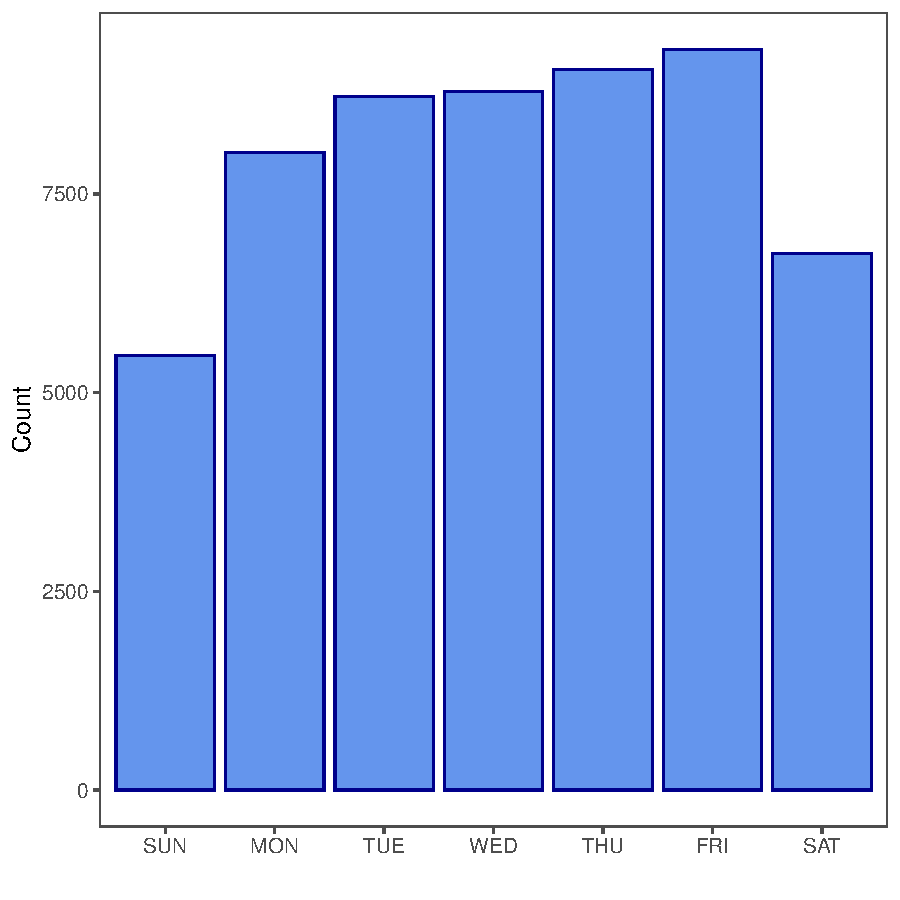
\includegraphics{variableinvestigation-002}


\subsection{Month of the Year}

\begin{Schunk}
\begin{Sinput}
> #making monthnumber column
> weatherdata[,"monthnumber"] = match(tolower(weatherdata$Month.Of.Year), 
+                             tolower(month.name))
> table(weatherdata$Month.Of.Year)
\end{Sinput}
\begin{Soutput}
  JANUARY  FEBRUARY     MARCH     APRIL       MAY      JUNE      JULY    AUGUST 
     5063      4728      4120      3825      4475      4735      5152      4907 
SEPTEMBER   OCTOBER  NOVEMBER  DECEMBER 
     4632      4836      4568      5095 
\end{Soutput}
\begin{Sinput}
> weatherdata %>%
+   ggplot(aes(x=Month.Of.Year)) +
+   geom_histogram(stat='count', colour='#00008b', fill='#6495ed') + 
+   xlab('') + 
+   ylab('Count') + 
+   scale_x_discrete(labels=(month.abb))
\end{Sinput}
\end{Schunk}
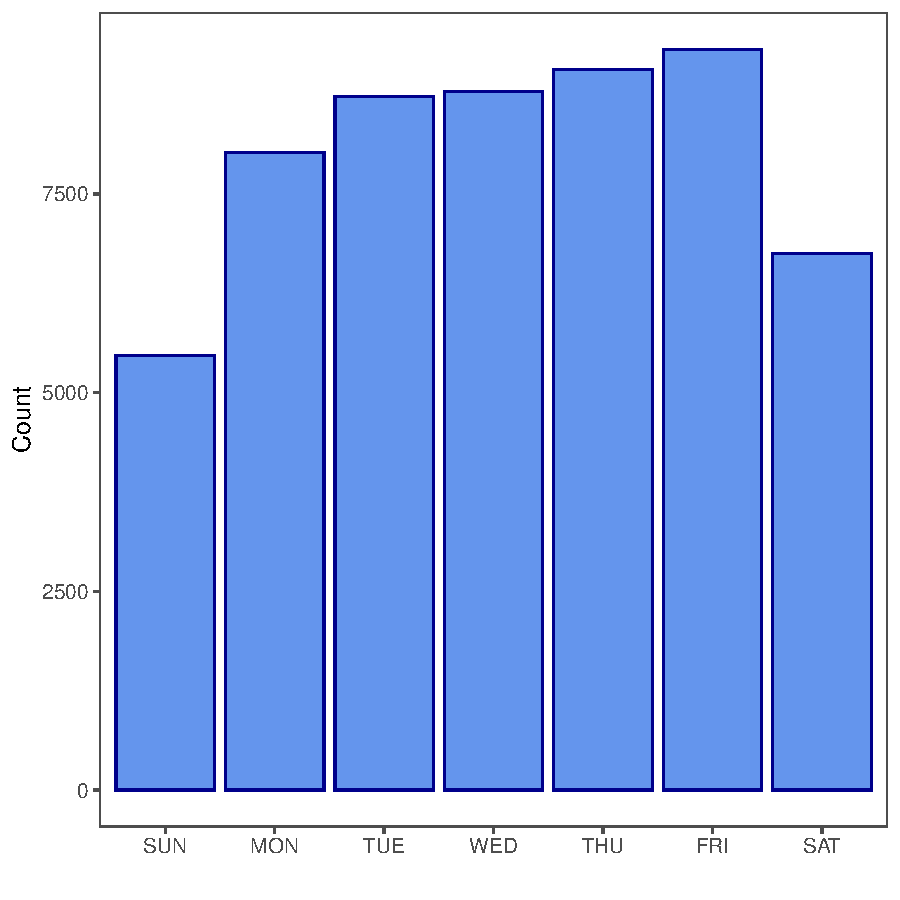
\includegraphics{variableinvestigation-003}





\section{Temperature}

\begin{Schunk}
\begin{Sinput}
> summary(weatherdata$Temp...C.)
\end{Sinput}
\begin{Soutput}
   Min. 1st Qu.  Median    Mean 3rd Qu.    Max.    NA's 
 -22.43    1.60   10.37   10.92   20.00   37.73      35 
\end{Soutput}
\begin{Sinput}
> weatherdata %>%
+   ggplot(aes(x=Temp...C.)) +
+   geom_histogram(colour='#00008b', fill='#6495ed', bins=20) + 
+   xlab('Temperature') + 
+   ylab('Count') + 
+   scale_x_continuous(labels = scales::label_number(suffix = "°C", accuracy=1), 
+                      limits = c(-40, 40)) 
\end{Sinput}
\end{Schunk}
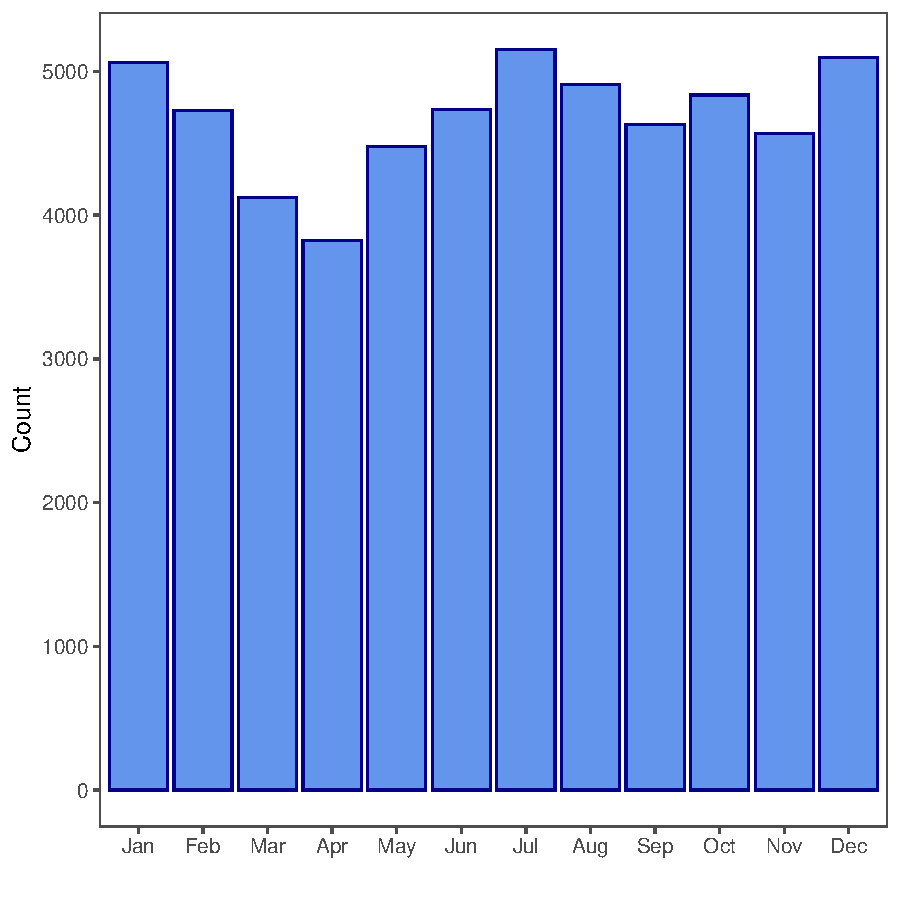
\includegraphics{variableinvestigation-004}

\begin{Schunk}
\begin{Sinput}
> weatherdata %>% 
+   ggplot(aes(x=monthnumber, y=Temp...C.)) + 
+   geom_boxplot(aes(x=Month.Of.Year), colour='#00008b', fill='#6495ed') + 
+   geom_smooth(stat = 'summary', alpha = 0.2, fill = '#6495ed', color = '#00008b',
+                 fun.data = median_hilow, fun.args = list(conf.int = 1)) +
+   #geom_line(stat='summary', fun='median', color='#00008b', lwd=1.2) + 
+   xlab('') + 
+   ylab('Temperature') + 
+   scale_x_discrete(labels=month.abb) + 
+   scale_y_continuous(labels = scales::label_number(suffix = "°C")) + 
+   theme(panel.grid.major.y = element_line(color = "#8ccde3",
+                                   size = 0.25,
+                                   linetype = 2))
\end{Sinput}
\end{Schunk}
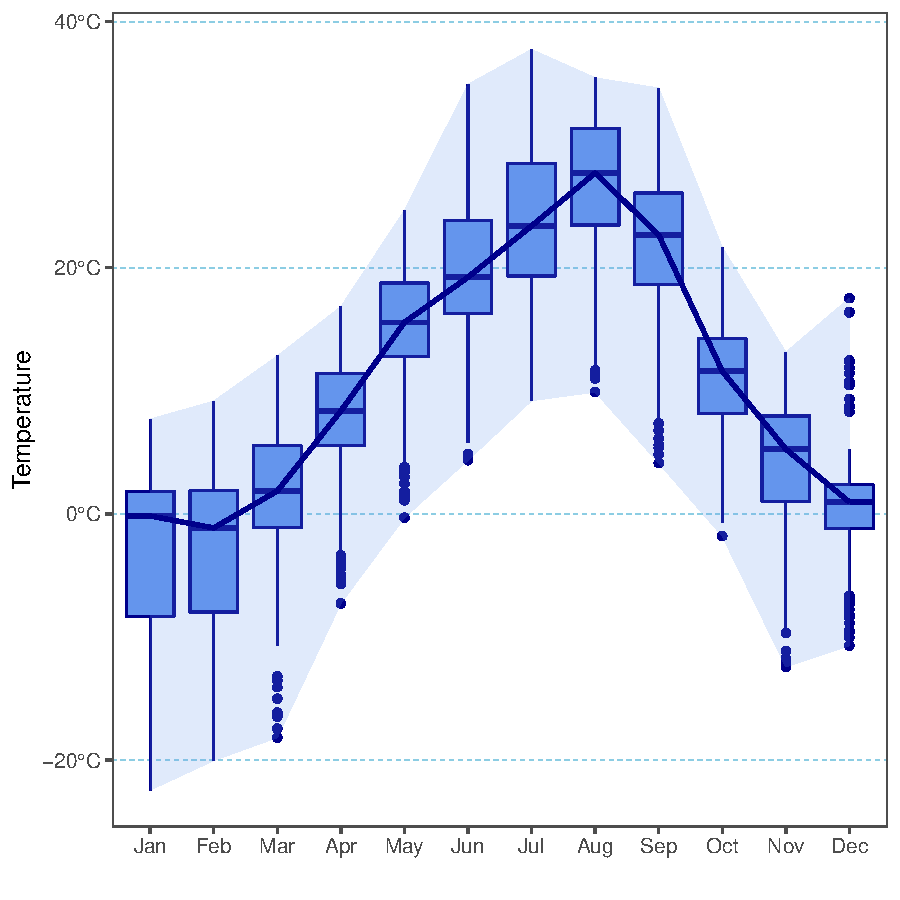
\includegraphics{variableinvestigation-005}






















\pagebreak
\section{Crash Severity}






\end{document}
